% Figure 4 composite (vector). Build: pdflatex fig4_assemble.tex
\documentclass[tikz,border=1mm]{standalone}
\usepackage{graphicx}\usepackage{helvet}\renewcommand{\familydefault}{\sfdefault}
\begin{document}
\begin{tikzpicture}[x=1mm,y=1mm]
  \useasboundingbox (0,0) rectangle (183,182);
  % row 1: a PDS-splits | b Pearson-splits | c null
  \node[anchor=north west,inner sep=0] at (3,178)  {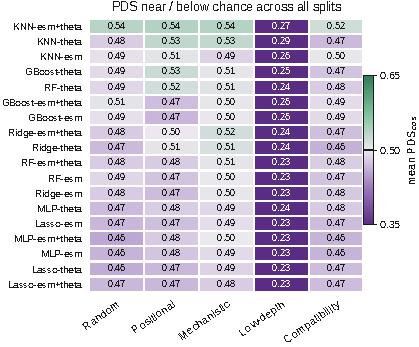
\includegraphics[width=58mm]{fig4a_pds_splits.pdf}};
  \node[anchor=north west,inner sep=0] at (64,178) {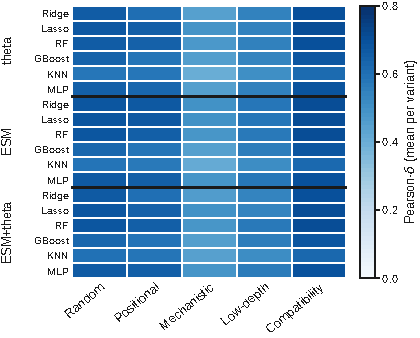
\includegraphics[width=58mm]{fig4b_pearson_splits.pdf}};
  \node[anchor=north west,inner sep=0] at (126,178){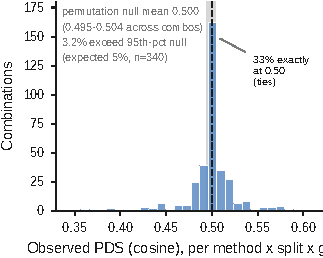
\includegraphics[width=54mm]{fig4c_null.pdf}};
  % row 2: d distance | e features | f gene x split
  \node[anchor=north west,inner sep=0] at (6,124)  {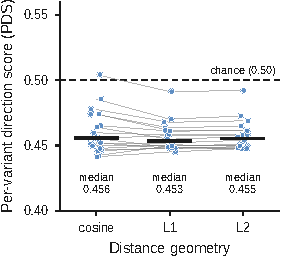
\includegraphics[width=50mm]{fig4d_distance.pdf}};
  \node[anchor=north west,inner sep=0] at (60,124) {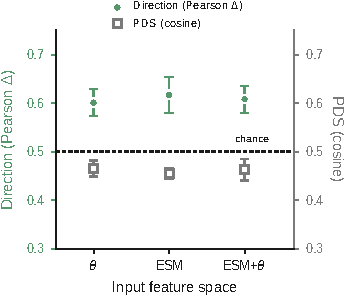
\includegraphics[width=58mm]{fig4e_features.pdf}};
  \node[anchor=north west,inner sep=0] at (122,124){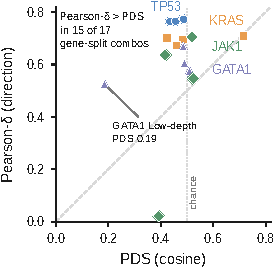
\includegraphics[width=50mm]{fig4f_gene_split.pdf}};
  % row 3: g external forest (hero) | h interface audit
  \node[anchor=north west,inner sep=0] at (4,70)  {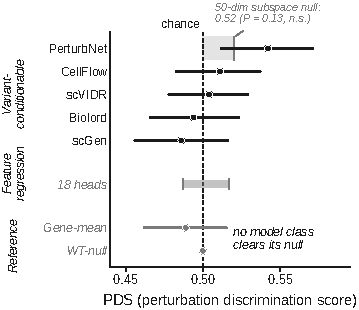
\includegraphics[width=66mm]{fig4g_external_forest.pdf}};
  \node[anchor=north west,inner sep=0] at (74,74) {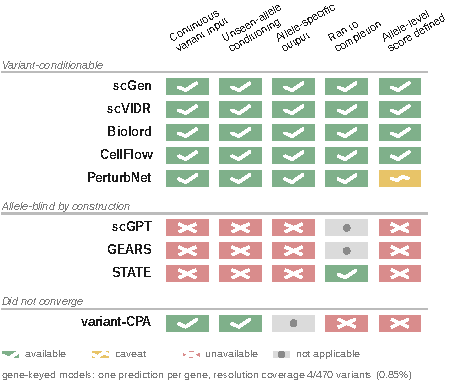
\includegraphics[width=78mm]{fig4h_interface.pdf}};
  % panel letters
  \tikzset{plab/.style={font=\bfseries\large,anchor=north west,inner sep=0}}
  \node[plab] at (0,181) {a};   \node[plab] at (61,181) {b};   \node[plab] at (123,181) {c};
  \node[plab] at (2,123) {d};   \node[plab] at (57,123) {e};   \node[plab] at (119,123) {f};
  \node[plab] at (1,69) {g};    \node[plab] at (71,69) {h};
\end{tikzpicture}
\end{document}
